%%%%%%%%%%%%%%%%%%%%%%%%%%%%%%%%%%%%%%%%%%%%%%%%%%%
%% P3: Phenomenology of Particle Physics                         
%%
%% Author:  André Rubbia                   		 
%%
%% Figure 18.17 Parton distribution functions assuming different models for the proton.
%%
%% This work is licensed under the Creative Commons Attribution 4.0 International License. 
%% To view a copy of this license, visit http://creativecommons.org/licenses/by/4.0/ or 
%% send a letter to Creative Commons, PO Box 1866, Mountain View, CA 94042, USA.
%%
%%%%%%%%%%%%%%%%%%%%%%%%%%%%%%%%%%%%%%%%%%%%%%%%%%%

\documentclass[a4paper,10pt]{article}

\usepackage[T1]{fontenc}
\usepackage[utf8]{inputenc}
\usepackage{lmodern}
\usepackage[labelfont=bf]{caption}
\usepackage{upgreek}
\usepackage{braket}

\usepackage{tikz}
\usepackage{pgfplots}
\pgfplotsset{compat=1.17}
\usepgfplotslibrary{ternary}
\usepgfplotslibrary{fillbetween}
\usepgfplotslibrary{external}

\def\d{\mathrm{d}}

\begin{document}

%%%%%%%%%%%%%%%   FIGURE  %%%%%%%%%%%%%%%%%%%%%%%%%%%%%%
\begin{figure}[htb]
\centering
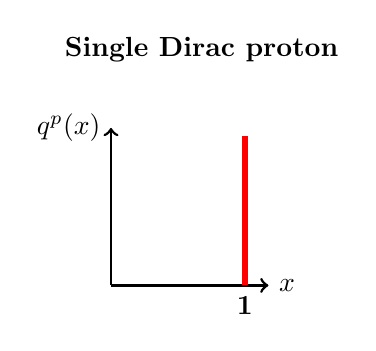
\begin{tikzpicture}[scale=1.0]
 \begin{scope}[shift={(0,0)}]
\draw[line width=1pt,black,->] (0,0)  -- +(2,0) node[right] {$x$};
\draw[line width=1pt,black,->] (0,0)  -- +(0,2) node[left] {$q^p(x)$};
\node at (1.15,3) {\textbf{Single Dirac proton}};
\node at (1.7,-0.25) {\textbf{1}};
\draw[line width=2pt,red] (1.7,0)  -- +(0,1.9);
\end{scope}
\end{tikzpicture}
%%%%%%%%%%%%%%%%%%%%%%%%%%
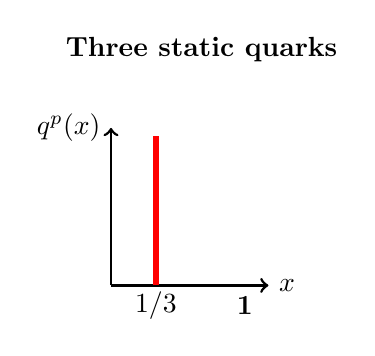
\begin{tikzpicture}[scale=1.0]
 \begin{scope}[shift={(2.5,0)}]
\draw[line width=1pt,black,->] (0,0)  -- +(2,0) node[right] {$x$};
\draw[line width=1pt,black,->] (0,0)  -- +(0,2) node[left] {$q^p(x)$};
\node at (1.15,3) {\textbf{Three static quarks}};
\node at (1.7,-0.25) {\textbf{1}};
\node at (0.57,-0.25) {\textbf{$1/3$}};
\draw[line width=2pt,red] (0.57,0)  -- +(0,1.9);
\end{scope}
\end{tikzpicture}
%%%%%%%%%%%%%%%%%%%%%%%%%%
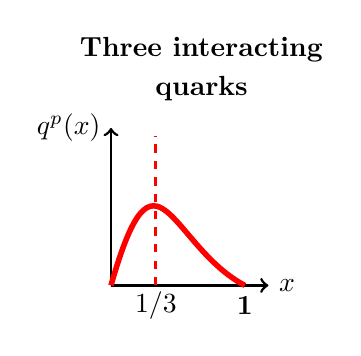
\begin{tikzpicture}[scale=1.0]
 \begin{scope}[shift={(5,0)}]
\draw[line width=1pt,black,->] (0,0)  -- +(2,0) node[right] {$x$};
\draw[line width=1pt,black,->] (0,0)  -- +(0,2) node[left] {$q^p(x)$};
\node at (1.15,3) {\textbf{Three interacting}};
\node at (1.15,2.5) {\textbf{quarks}};
\node at (1.7,-0.25) {\textbf{1}};
\node at (0.57,-0.25) {\textbf{$1/3$}};
\draw[line width=1pt,red,dashed] (0.57,0)  -- +(0,1.9);
\draw[line width=2pt,red] (0,0)  .. controls (0.57,2) and (0.75,0.5) .. (1.7,0);
\end{scope}
\end{tikzpicture}
%%%%%%%%%%%%%%%%%%%%%%%%%%
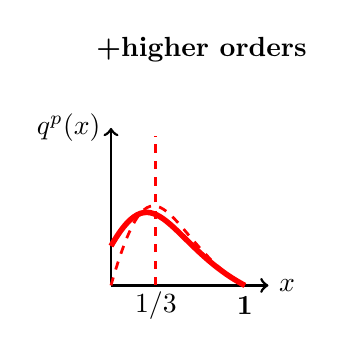
\begin{tikzpicture}[scale=1.0]
 \begin{scope}[shift={(7.5,0)}]
\draw[line width=1pt,black,->] (0,0)  -- +(2,0) node[right] {$x$};
\draw[line width=1pt,black,->] (0,0)  -- +(0,2) node[left] {$q^p(x)$};
\node at (1.15,3) {\textbf{+higher orders}};
\node at (1.7,-0.25) {\textbf{1}};
\node at (0.57,-0.25) {\textbf{$1/3$}};
\draw[line width=1pt,red,dashed] (0.57,0)  -- +(0,1.9);
\draw[line width=1pt,red,dashed] (0,0)  .. controls (0.57,2) and (0.75,0.5) .. (1.7,0);
\draw[line width=2pt,red] (0,0.5)  .. controls (0.57,1.5) and (0.75,0.5) .. (1.7,0);
\end{scope}
\end{tikzpicture}
%%%%%%%%%%%%%%%%%%%%%%%%%%
\caption{Parton distribution functions assuming different models for the proton.}
\end{figure}
%%%%%%%%%%%%%%%  END FIGURE  %%%%%%%%%%%%%%%%%%%%%%%%%%%%%%
%

\end{document}
